\documentclass[red]{beamer}

%\usetheme{default}
\usetheme{Darmstadt}
%\usecolortheme{beaver}

\setbeamertemplate{navigation symbols}{} 
\useoutertheme[subsection=false]{miniframes}

%\usepackage{iwona}

\usepackage{amsfonts}
\usepackage{amsmath}
\usepackage{amsthm}
\usepackage{amssymb}
\usepackage{graphicx}

\usepackage[american]{babel}
\usepackage{csquotes}
\usepackage[style=apa,natbib=true,backend=biber]{biblatex}
\DeclareLanguageMapping{american}{american-apa}
\addbibresource{Polarization.bib}
% smaller references
\renewcommand*{\bibfont}{\scriptsize}

\newcommand{\vitem}{\vfill\item}

\usepackage{hyperref}
\ExecuteBibliographyOptions{doi=false}
\newbibmacro{string+doi}[1]{%
  \iffieldundef{doi}{#1}{\href{http://dx.doi.org/\thefield{doi}}{#1}}}
\DeclareFieldFormat{title}{\usebibmacro{string+doi}{\mkbibemph{#1}}}
\DeclareFieldFormat[article]{title}{\usebibmacro{string+doi}{\mkbibquote{#1}}}

\title[Tasks and Polarisation]{Is Technology Polarising Australia's Work Force?}
\author{Alex Cooper \\ Honours Candidate \\ Macquarie University}
%\institution[Macquarie University]{Macquarie University}
\date{August 2013}

\setlength{\itemsep}{\fill}

\usepackage[absolute,overlay]{textpos}
\pgfdeclareimage[height=1.4cm]{fg:logo}{logo.pdf}
%\logo{
\includegraphics[height=1.4cm]{logo.pdf}}
%\useouterframe{subsection=false}

\begin{document}
%
\begin{frame}[plain]
\titlepage
\begin{textblock*}{\textwidth}(3.2in,3in) 
  \pgfuseimage{fg:logo} 
\end{textblock*} 
\end{frame}

\section{Motivation}

\subsection{Inequality Chart}
\begin{frame}[c]
\frametitle{Wage inequality has risen since the 1980s}
\begin{center}
  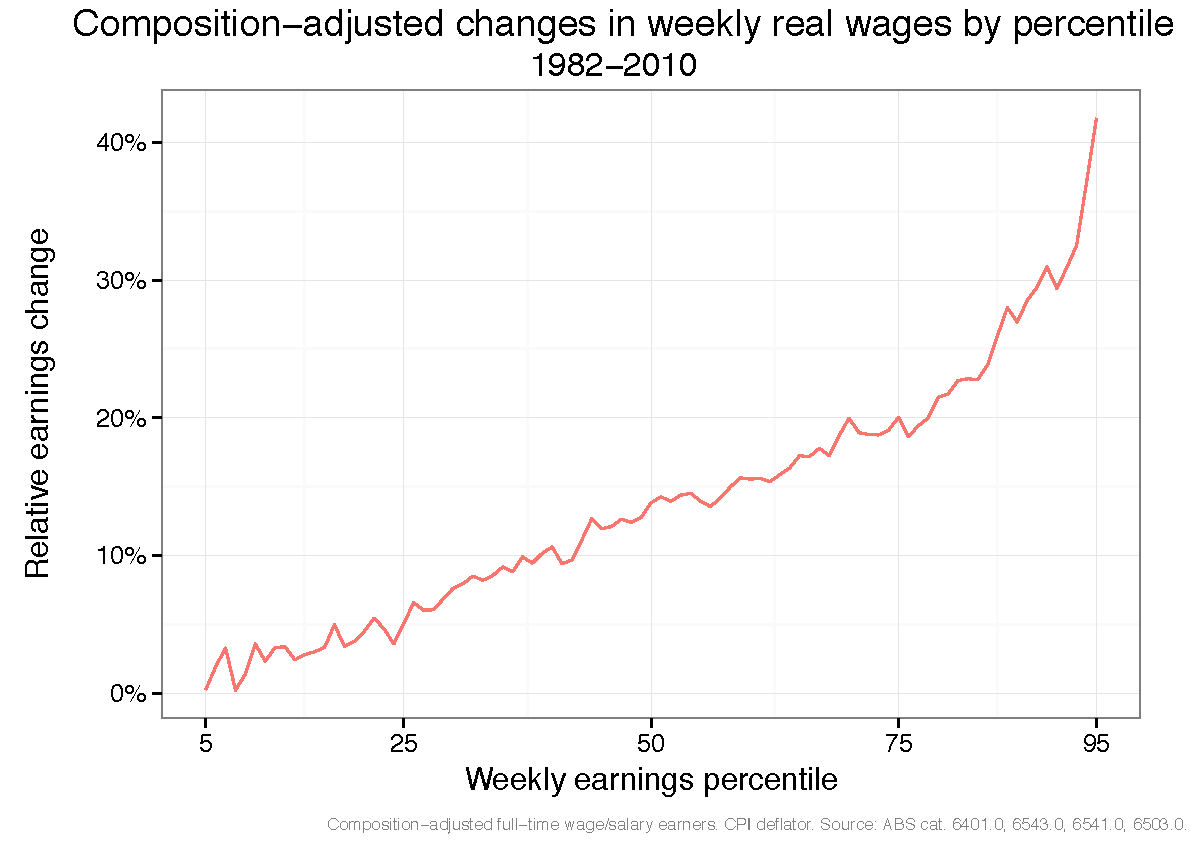
\includegraphics[width=\textwidth]{slides_fig/quantile_growth_percent.pdf}
\end{center}
\end{frame}

\begin{frame}[c]
\frametitle{Real cost of computation has decreased exponentially}
\begin{center}
  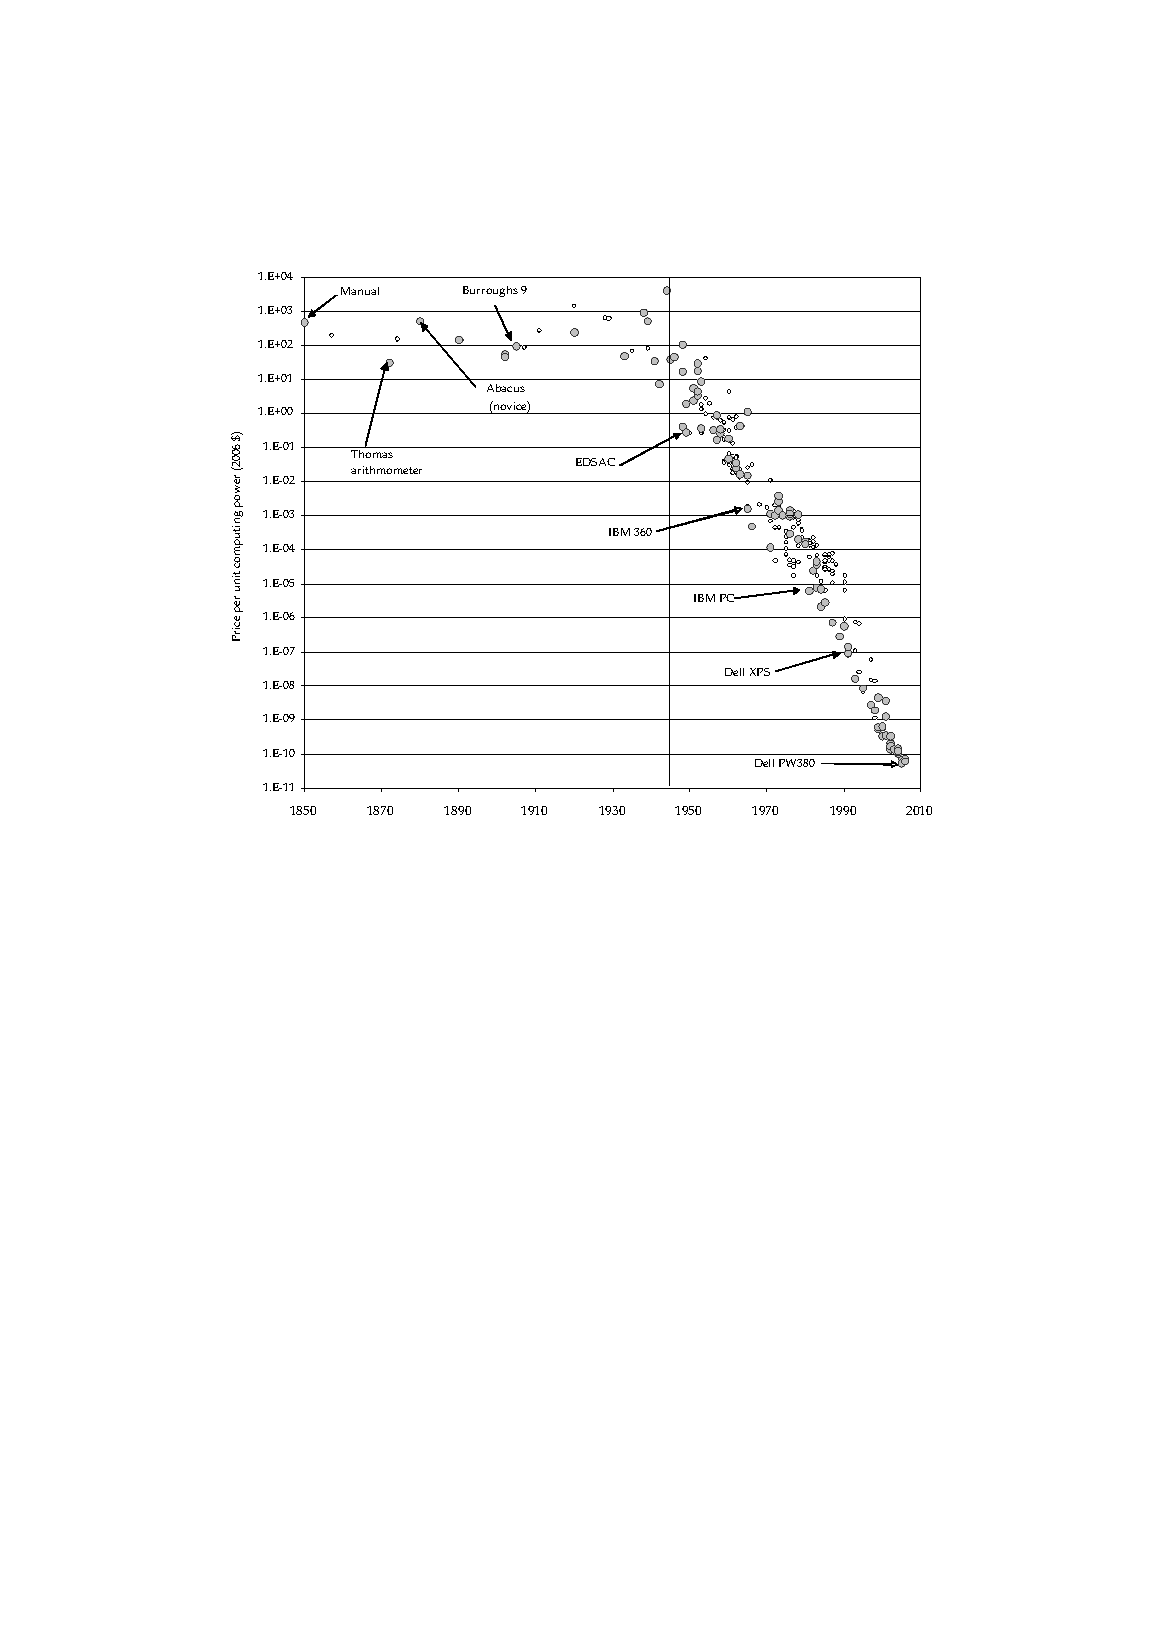
\includegraphics[width=0.8\textwidth]{slides_fig/nordhaus_2007.pdf}
\end{center}
Price per computation/second, 2006 USD (Nordhaus 2007)
\end{frame}

\subsection{Outline}
\begin{frame}[c]
\frametitle{Does technological change explain rising inequality?}
Three approaches:
\begin{enumerate}
\vfill\item The `canonical' model: skill-biased technical change (SBTC)
\vfill\item The relationship between ICT investment and occupational changes
\vfill\item Further research: job `task content' and wages
\end{enumerate}
\end{frame}

\section{Skill-biased technical change}
\subsection{Canonical Model}
\begin{frame}[c]
\frametitle{The `canonical model:' skill-biased technical change}
\begin{center}
  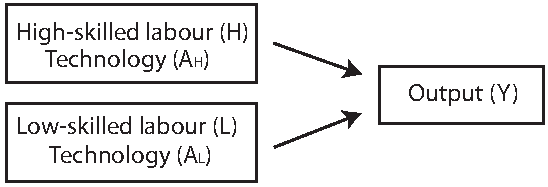
\includegraphics[width=\textwidth]{slides_fig/CES.pdf}
\end{center}
Production function:
\begin{equation*}
  \label{eq:cobbdoug}
  F = \left[\left(A_LL\right)^{\frac{\sigma - 1}{\sigma}}
            + \left(A_HH\right)^{\frac{\sigma - 1}{\sigma}}
          \right]^\frac{\sigma}{(\sigma-1)}
\end{equation*}
We assume $\sigma>1$.
\end{frame}

\begin{frame}
\frametitle{The `canonical model:' skill-biased technical change}
\begin{itemize}
\item When high-skilled technology is increasing, {\em ceteris paribus},
  \begin{itemize}
  \item Increasing inequality, driven by skill demand.
  \item Rising college/education premium.
  \item Monotone wage growth in skills.
  \end{itemize}
\vspace{1cm}
\item Empirically successful, e.g.
  \begin{itemize}
  \item Katz and Murphy (1992)
  \item Card and Lemieux (2001)
  \end{itemize}
\end{itemize}
\end{frame}

\subsection{Results: wage premium}
\begin{frame}
  \frametitle{College wage premium}
  \begin{center}
    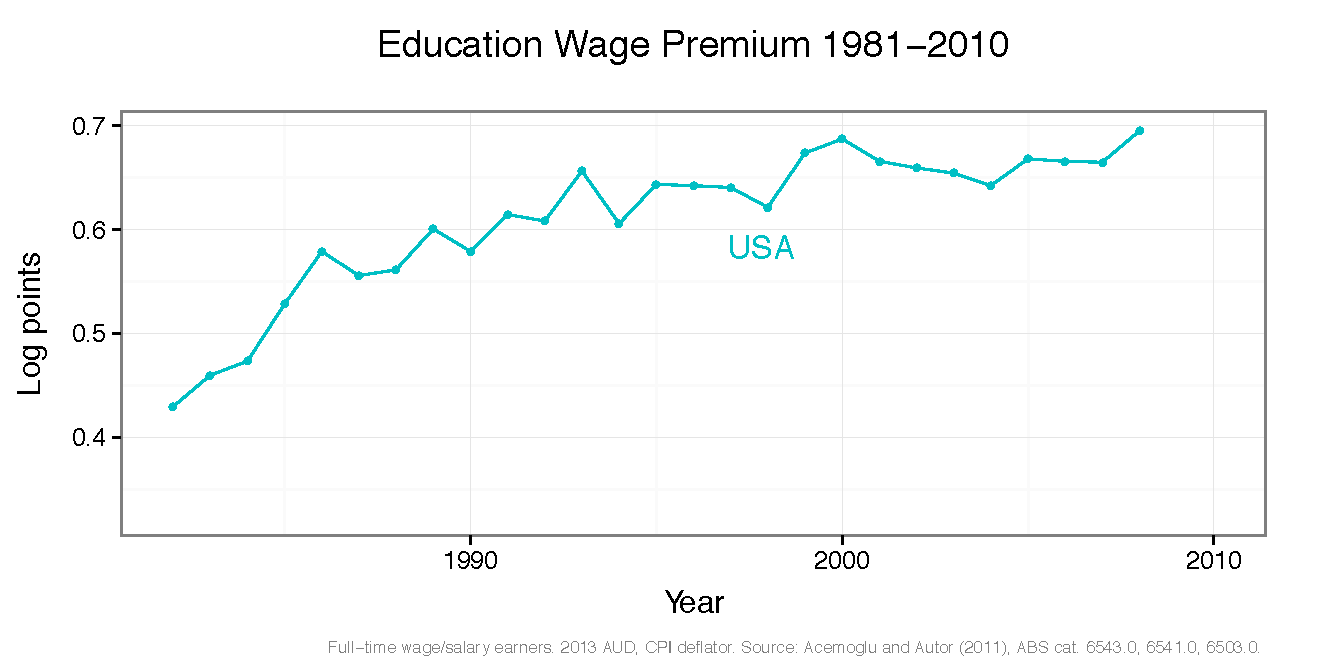
\includegraphics[width=\textwidth]{slides_fig/ed_premium_us.pdf}
  \end{center}
\end{frame}

\begin{frame}
  \frametitle{College wage premium}
  \begin{center}
    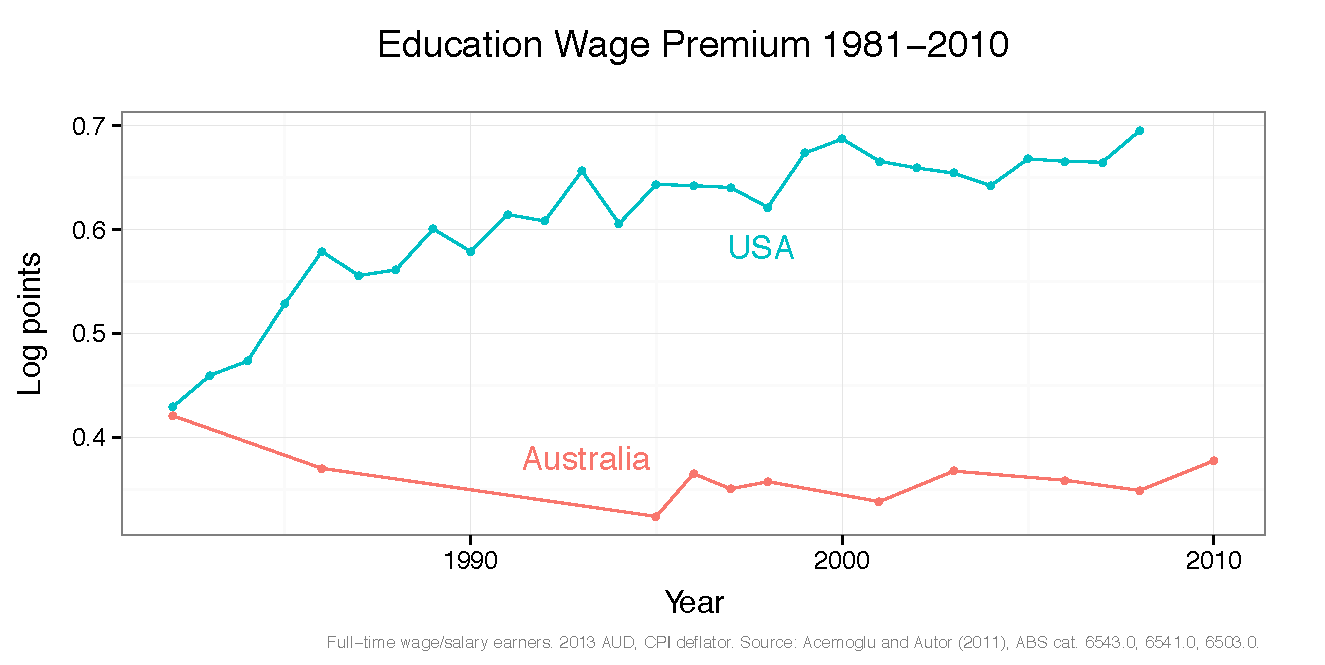
\includegraphics[width=\textwidth]{slides_fig/ed_premium.pdf}
  \end{center}
\end{frame}

\subsection{Results: non-monotone wage growth}
\begin{frame}{Non-monotone wage growth in time}
  \begin{center}
    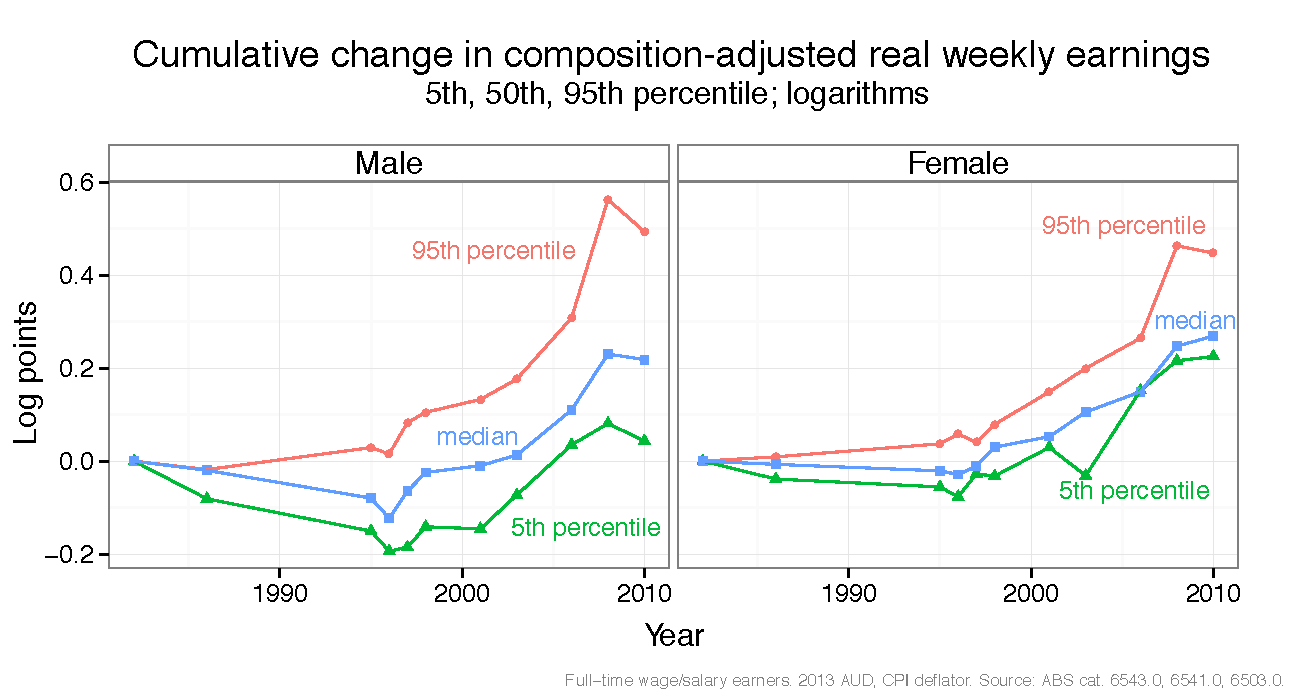
\includegraphics[width=\textwidth]{slides_fig/wage_change_time.pdf}
  \end{center}
\end{frame}

\begin{frame}{Wage growth by wage percentile and sex}
  \begin{center}
    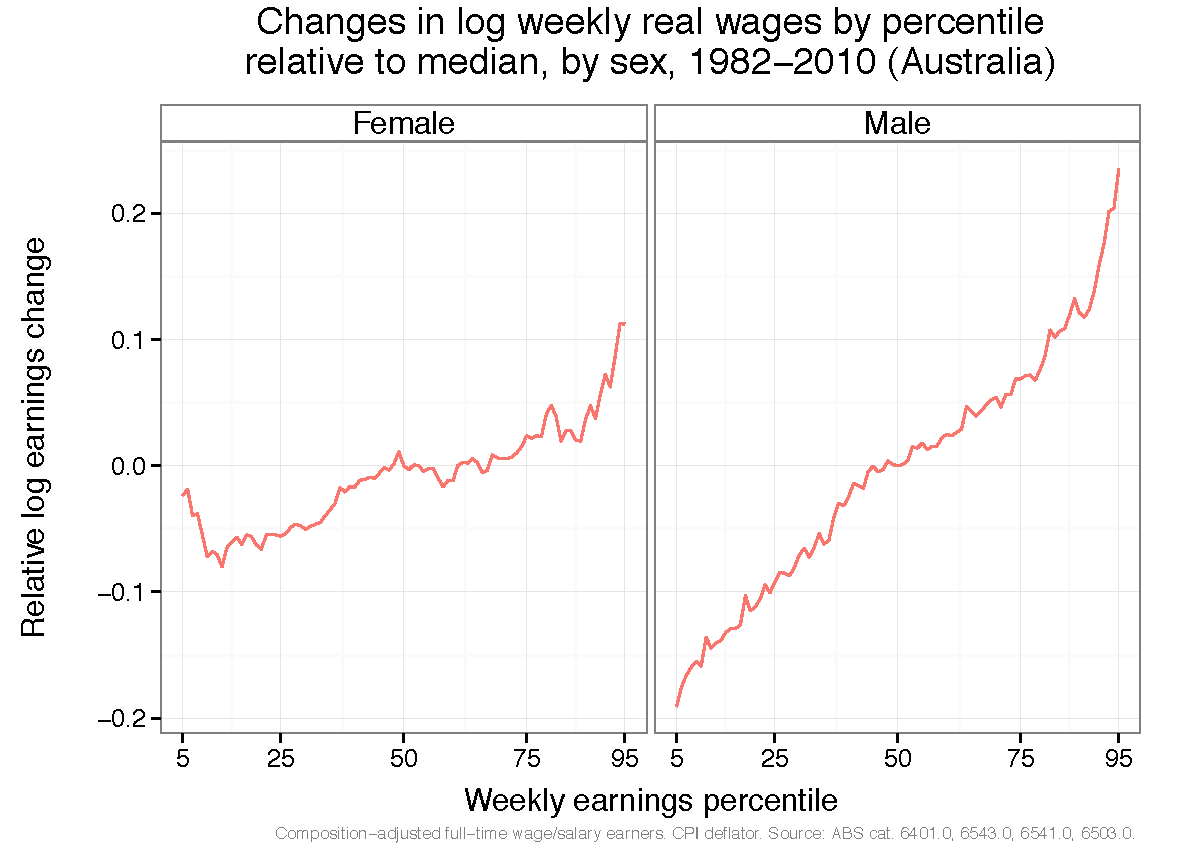
\includegraphics[width=\textwidth]{slides_fig/quantile_growth_mf.pdf}
  \end{center}
\end{frame}

\subsection{Results: summary}
\begin{frame}
  \frametitle{Failure of the SBTC model: summary}
  \begin{itemize}
  \vitem No clear `college premium' in Australia (see Coelli 2007)
  \begin{itemize}
  \vitem Education a poor proxy for skills (`credentialism')?
  \vitem Expanding supply of college-educated workers?
  \vitem Does not appear to be driving inequality trend
  \end{itemize}
  \vitem Wage growth is non-monotone
  \vitem Non-monotone wage growth across earnings spectrum
  \vitem Despite composition adjustment, male and female wage profiles differ
  \end{itemize}
\end{frame}

\subsection{One explanation?}
\begin{frame}{Could job composition explain the trend?}
  \begin{center}
    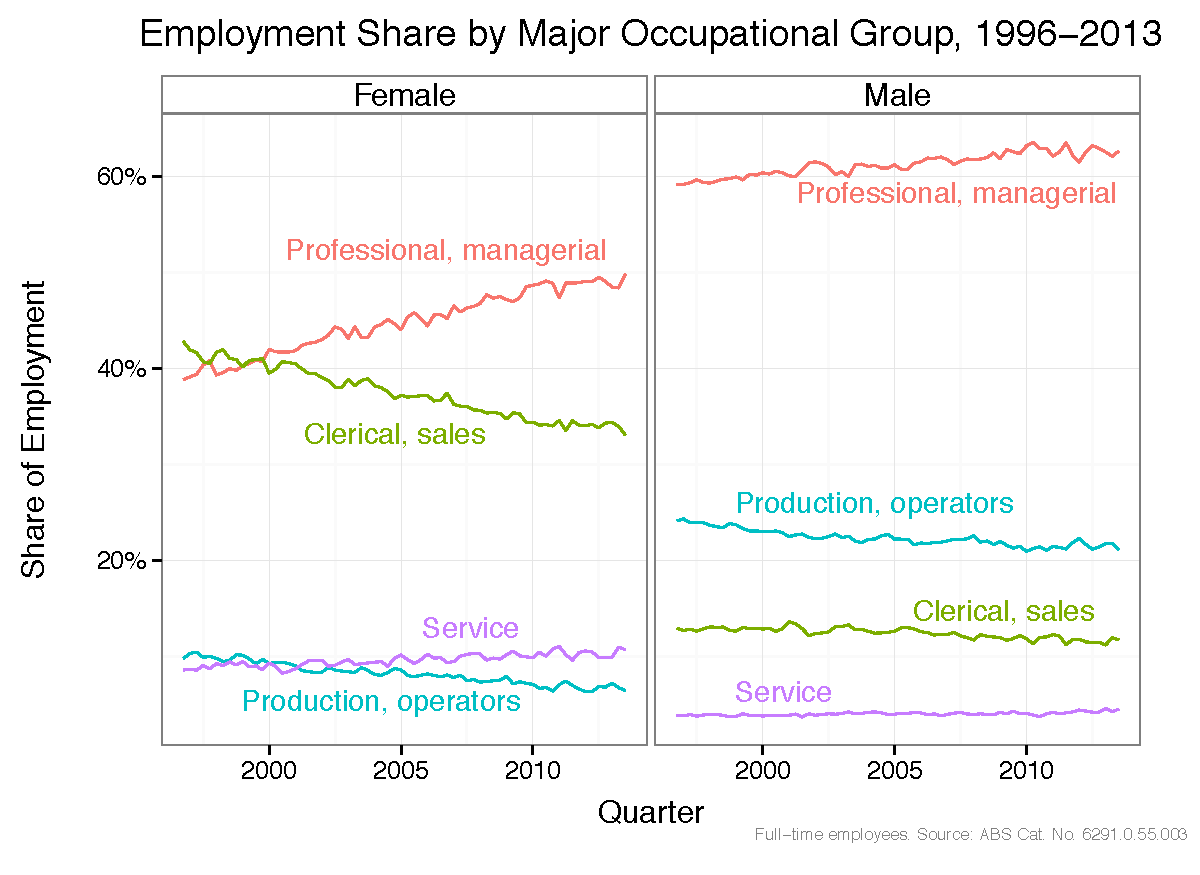
\includegraphics[width=\textwidth]{slides_fig/occ_share_sex.pdf}
  \end{center}
\end{frame}

\section{The `task approach'}
\subsection{Substitutive technology}
\begin{frame}[c]
\frametitle{The `task approach'}
Autor, Levy, and Murnane (QJE 2003)
\vfill
\begin{itemize}
\item Recall `canonical' approach: factors produce output via 
       production function $F$
\[ \text{capital, labour} \overset{F}{\longrightarrow} \text{output}. \]
\begin{itemize}
\item Technology is factor-augmenting (labour and capital complements)
\vfill
\end{itemize}
\vitem ALM: factors produce tasks, which produce output:
\[ \text{capital, labour} \longrightarrow \text{tasks} \overset{F}{\longrightarrow} \text{output}. \]
\begin{itemize}
\item Technology can be complementary or a substitute
\end{itemize}
\end{itemize}
\end{frame}

\subsection{A simple test}
\begin{frame}
\frametitle{The `task approach'}
\begin{itemize}
\vitem Jobs have different task content
\vitem Capital can substitute for only certain `routine' tasks.
  \begin{itemize}
  \item Typically `middle-skill,' like clerical work
  \end{itemize}
\vitem Michaels {\em et al} (2013) expand the canonical model with `middle-skilled' labour
  \begin{itemize}
  \item Three kinds of labour: $H$, $M$, $L$, and ICT capital $C$. 
  \item Capital $C$ and $M$ are perfect substitutes
  \item Middle-skilled workers compete with ICT capital
  \end{itemize}
\end{itemize}
\end{frame}

\begin{frame}[c]
\frametitle{The `task approach'}
\begin{itemize}
\item The canonical approach\\
\begin{center}
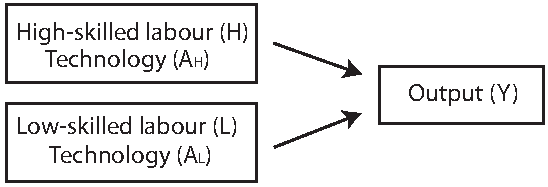
\includegraphics[width=2in]{slides_fig/CES.pdf}
\end{center}
\item The task approach\\
\begin{center}
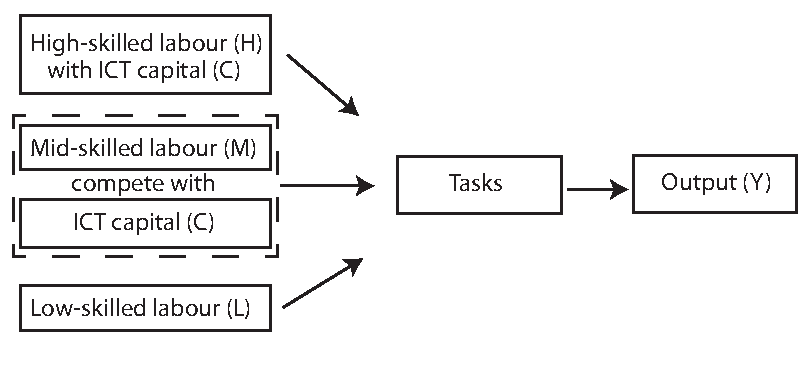
\includegraphics[width=3in]{slides_fig/CES_tasks.pdf}
\end{center}
\end{itemize}
\end{frame}

\begin{frame}[c]
  \frametitle{A simple test (Michaels {\em et al.} 2013)}
Production function with three types of labour and ICT capital $C$:
$$
Y = \left[
  \underbrace{(A_LL)^\frac{\sigma-1}{\sigma}}_{\text{low}}
  +
  \underbrace{(A_MM + C)^\frac{\sigma-1}{\sigma}}_{\text{medium}}
  +
  \underbrace{((A_HH)^\mu + C^\mu)^\frac{\sigma-1}{\mu\sigma}}_{\text{high}}
  \right]^\frac{1}{\sigma-1}
$$
  \begin{itemize}
  \item Comparative statics: if $C$ increases exogenously, then: 
  \begin{itemize}
  \item high-skilled wage share should increase, and 
  \item medium-skilled wage share should decrease.
  \end{itemize}
  \vitem We form three groups of occupations:
  \begin{itemize}
  \item High-skilled---managers and professionals
  \item Middle-skilled---clerical and sales workers
  \item Low-skilled---labourers, tradespersons, transport workers
  \end{itemize}
  \vitem For each industry we compute:
  \begin{itemize}
  \item Skill group wage share (Survey of Income and Housing)
  \item ICT capital stock/value added ratio (National Accounts)
  \end{itemize}
\end{itemize}
\end{frame}

\begin{frame}[c]
  \frametitle{ICT capital (equipment) and wage shares by group}
\begin{center}
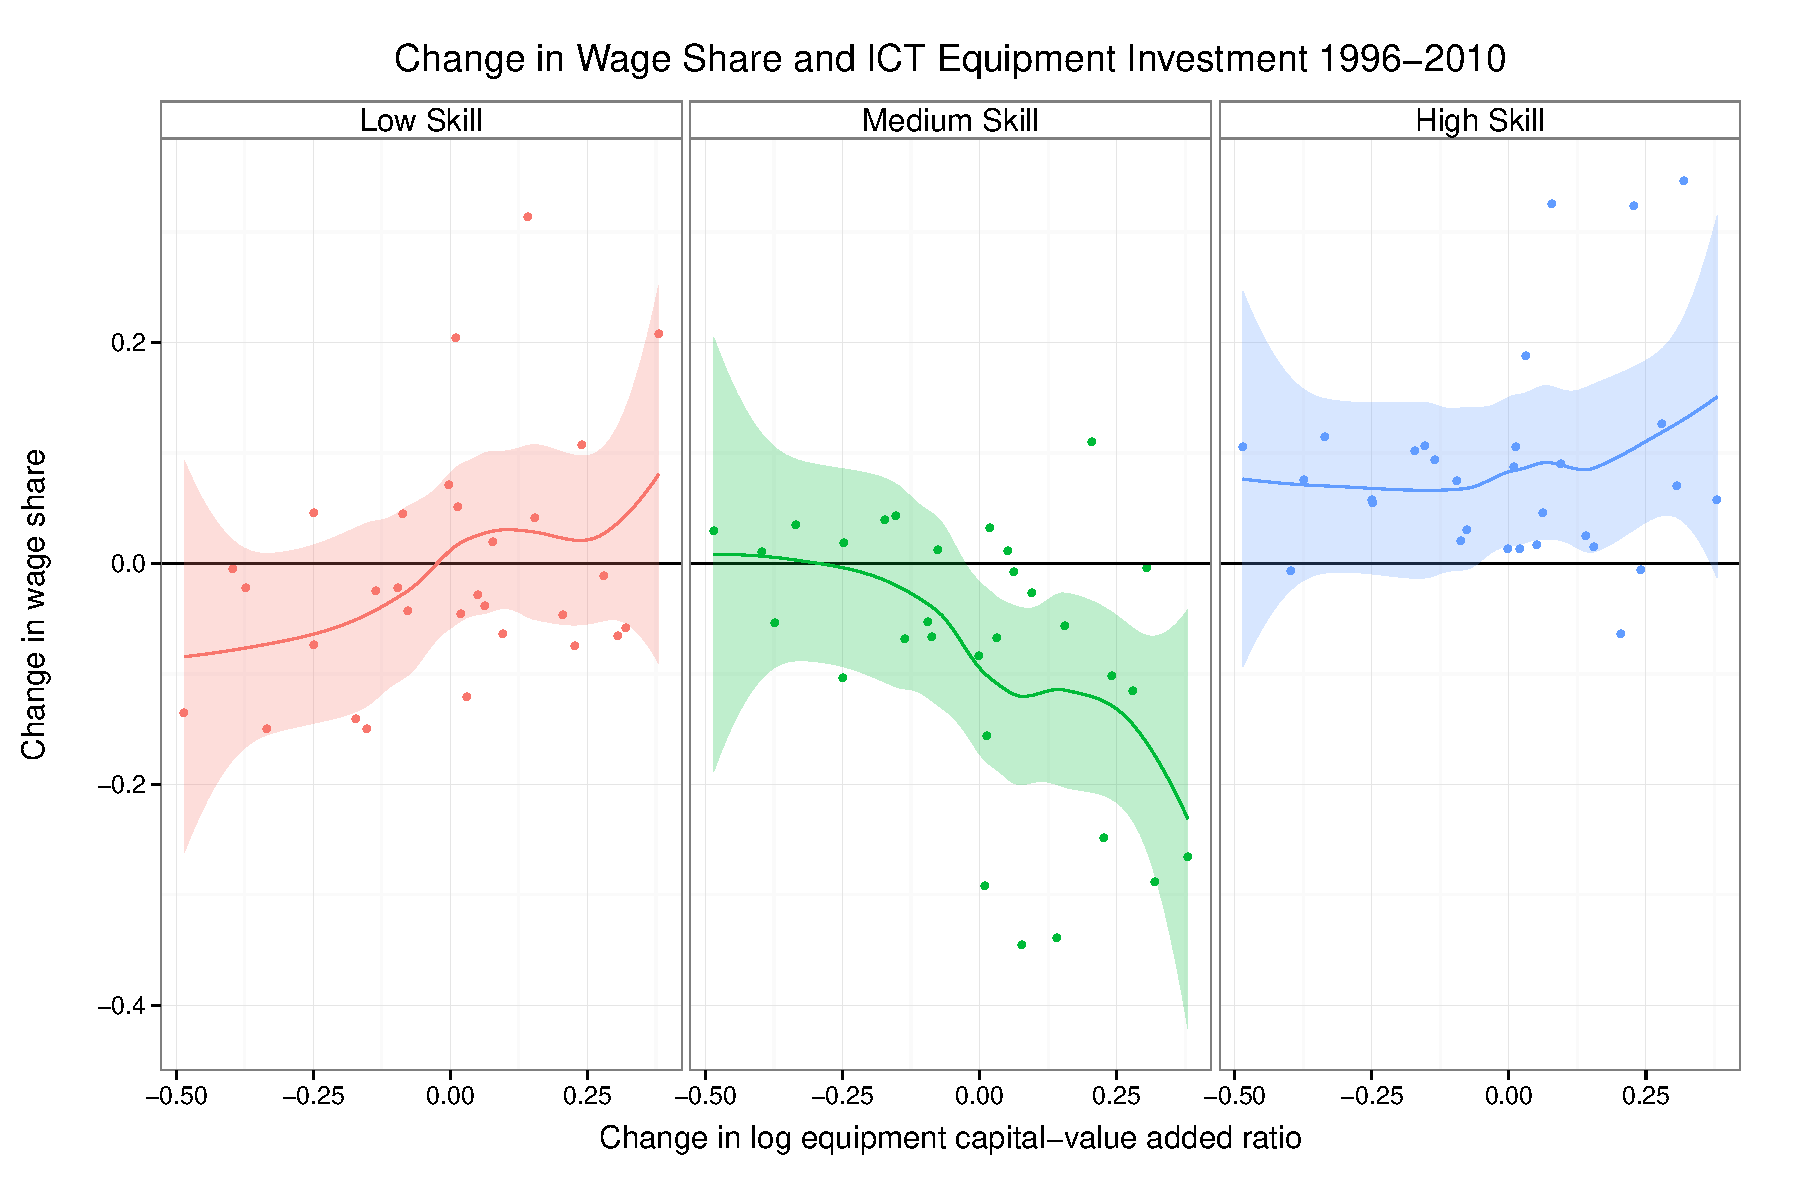
\includegraphics[width=\textwidth]{slides_fig/wage_share_equipment_skill.pdf}
\end{center}
\end{frame}

\begin{frame}[c]
  \frametitle{Problems with this result}
  \begin{itemize}
    \vitem Model gives only {\em wage share}, not {\em wage}
    \vitem ICT investment endogenous, with no obvious instruments
    \vitem Tests have low power
    \begin{itemize}
      \item few industry groups
      \item occupational groupings too simplistic
    \end{itemize}
    \vitem Conflicting results with other ICT capital measures 
           (software, computer peripherals)
    \vitem No obvious way to deflate ICT capital for consistent comparison
  \end{itemize}
\end{frame}

\subsection{A more sophisticated approach}
\begin{frame}
  \frametitle{A more sophisticated approach}
  Following Firpo, Fortin, \& Lemieux (2011),
  \begin{itemize}
  \vitem Labour market as Roy model
    \begin{itemize}
    \item Self-selection into occupations by comparative advantage
    \end{itemize}
  \vitem Assume that ICT investment reduces demand for `routine' and `off-shoreable' occupations
  \vitem For these occupations, we predict:
    \begin{itemize}
    \item high-quality workers self-select out of these occupations
    \item a wage compression in these occupations at higher quantiles
    \end{itemize}
  \end{itemize}
\end{frame}

\begin{frame}
  \frametitle{Data}
  \begin{enumerate}
  \item O*NET: Occupational task database
    \begin{itemize}
    \item Developed by US Department of Labor
    \item Details work activities by occupation
    \end{itemize}
    \vspace{10pt}
  \item David Autor's work type data categories
    \begin{itemize}
    \item Routine/non-routine and `off-shoreable'
    \item Manually mapped to ANZSCO categories
    \end{itemize}
    \vspace{10pt}
  \item Australian Bureau of Statistics
    \begin{itemize}
    \item Census of Population and Housing for wages and occupations
    \end{itemize}
  \end{enumerate}
\end{frame}

\begin{frame}
\frametitle{O*NET Data Example}
\begin{table}[htbp]
\begin{tabular}{|p{2cm}|p{1.65cm}|p{1.5cm}|p{1.5cm}|p{1.5cm}|}
\hline
{Job Title} & {Gather Data} & {Analyze Data} & {\small Think Creatively} & {Handle Moving Objects} \\ \hline
{CEOs} & 5.03 & 4.82 & 5.1 & 1.1  \\ \hline
{Economists} & 5.88 & 6.58 & 5.38 & 0.54 \\ \hline
{Dancers} & 3.88 & 1.96 & 4.37 & 2.63 \\ \hline
{Programmers} & 4.91 & 5.05 & 5.96 & 0.44 \\ \hline
{Tellers} & 2.91 & 2.65 & 2.21 & 2.74 \\ \hline
{Surgeons} & 5.72 & 5.49 & 4.67 & 3.62 \\ \hline
{Bakers} & 2.8 & 3.29 & 2.93 & 5.06 \\ \hline
{Receptionists} & 3.1 & 2.45 & 2.54 & 2.88 \\ \hline
{Typists} & 4.35 & 1.52 & 3.9 & 1.43 \\ \hline
\end{tabular}
\caption{O*NET Work Activity Example (Levels, Scale 0--7)}
\label{onetex}
\end{table}
\end{frame}

\section*{References}

\begin{frame}
  \frametitle{Summary}
  \begin{itemize}
  \vitem Skill-biased technical change does not appear to explain widening inequality in Australia
  \vitem Changes in occupational composition seem important
  \vitem Correlation between `polarisation' and ICT capital
  \vitem Further work will focus on changes in wage structure and `task content' of jobs
  \end{itemize}
\end{frame}

\begin{frame}
  \begin{center}
    Questions
    \vspace{1cm}

    and
    \vspace{1cm}

    I'd love your feedback.
  \end{center}
\end{frame}

\begin{frame}
\frametitle{References}
%\printbibliography
{ \scriptsize
Acemoglu, D., \& Autor, D. H. (2011). Skills, Tasks and Technologies: Implications for Employment and Earnings. In D. Card \& O. Ashenfelter (Eds.), Handbook of labor economics, volume 4, part b (Chap. 12, Vol. Volume 4, pp. 1043–1171). Elsevier
\vfill

Autor, D. H., Levy, F., \& Murnane, R. J. (2003). “The skill content of recent technological change: An empirical exploration.” The Quarterly Journal of Economics, 118(4), 1279–1333.
\vfill

Card, D., \& Lemieux, T. (2001, May). “Can Falling Supply Explain the Rising Return to College for Younger Men? A Cohort-Based Analysis.” The Quarterly Journal of Economics, 116(2), 705–746
\vfill

Firpo, S., Fortin, N., \& Lemieux, T. (2011). Occupational tasks and changes in the wage structure. Institute for the Study of Labor.
\vfill

Katz, \& Murphy, K. J. (1992). “Changes in Relative Wages, 1963-1987: Supply and Demand Factors.” Quarterly Journal of Economics, 107, 35–78.
}
\end{frame}

\begin{frame}
  \begin{center}
    Spare Slides
  \end{center}
\end{frame}

\begin{frame}[c]
  \frametitle{ICT capital (software) and wage shares}
\begin{center}
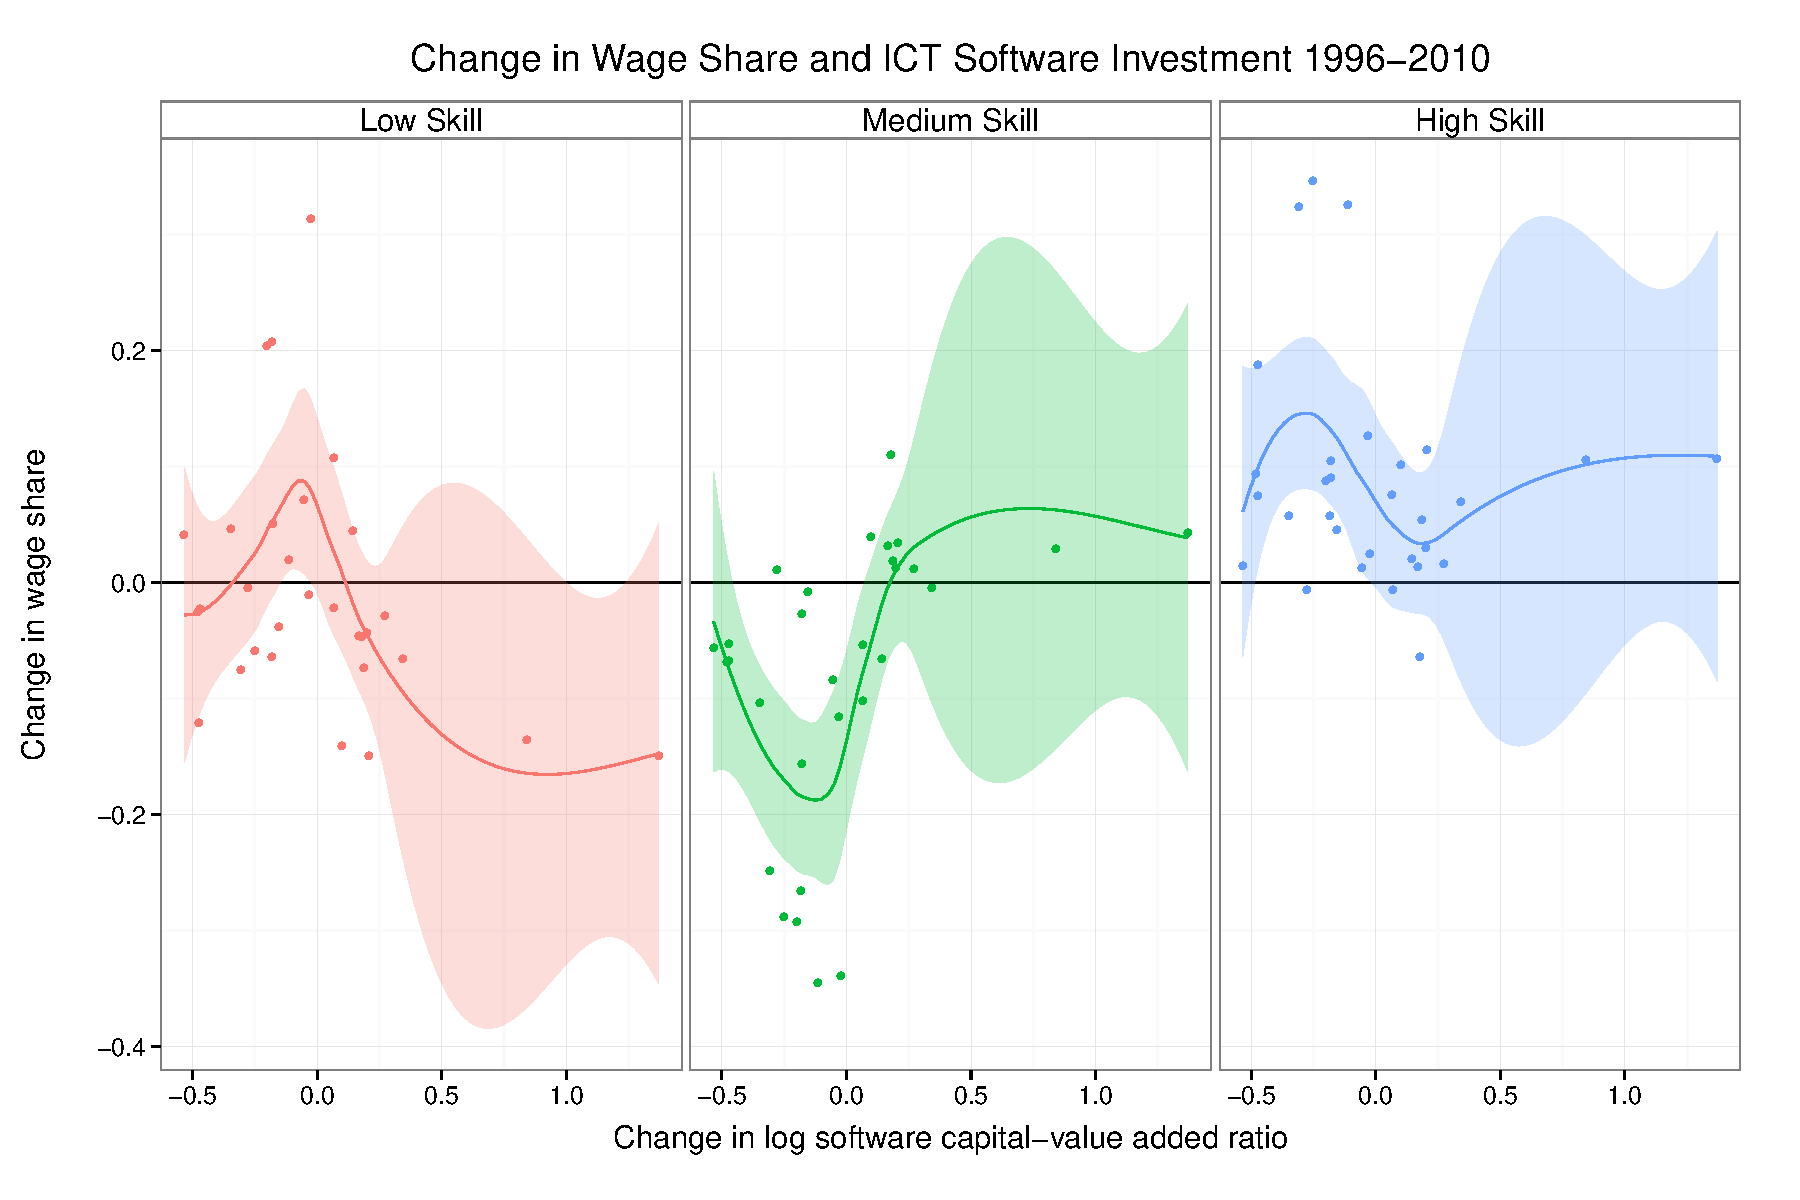
\includegraphics[width=\textwidth]{slides_fig/wage_share_software_skill.pdf}
\end{center}
\end{frame}

\begin{frame}[c]
  \frametitle{ICT capital (computers and peripherals) and wage shares}
\begin{center}
  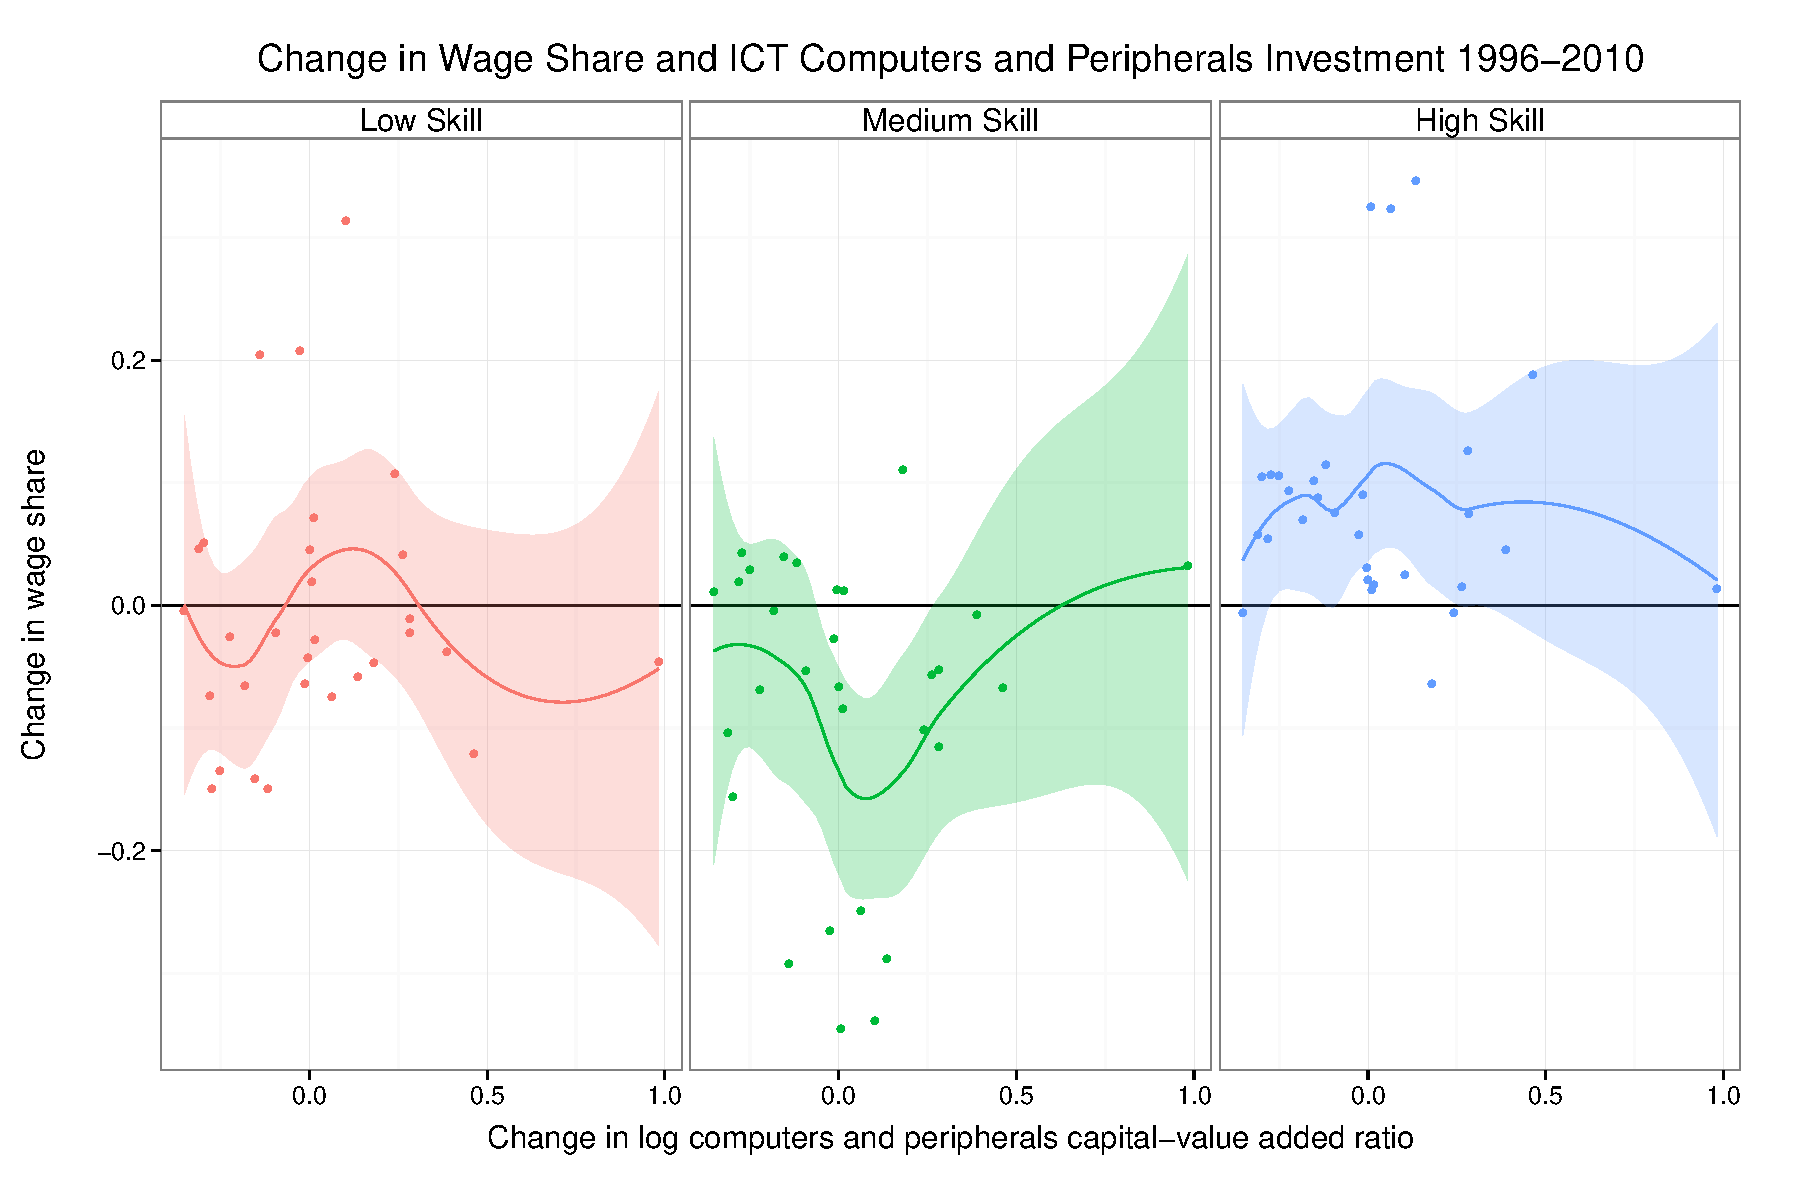
\includegraphics[width=\textwidth]{slides_fig/wage_share_peripherals_skill.pdf}
\end{center}
\end{frame}

\end{document} 
